\input{./_path-to-root.ltx}
\documentclass[\PathToRoot/\ProjectName]{subfiles}
\standaloneTableSetup % tex4ht compatible cross-reference setup
\whenstandalone{\externaldocument{\PathToRoot/\ProjectName}} % standalone: enable cros
\begin{document}

% Add clear separation from any preceding content
\vspace{1em}
\FloatBarrier 

\begin{figure}[H] 
  \centering
  \caption{Policy effectiveness during recessions with aggregate demand effects}
  \whenintegrated{\label{fig:Policyrelrecession}} 
  \noindent\begin{minipage}{\textwidth}
    \centering
    \begin{subfigure}[b]{.32\linewidth}
      \centering
      % Original path: \PathToRoot/Code/HA-Models/FromPandemicCode/Figures/recession_Check_relrecession
      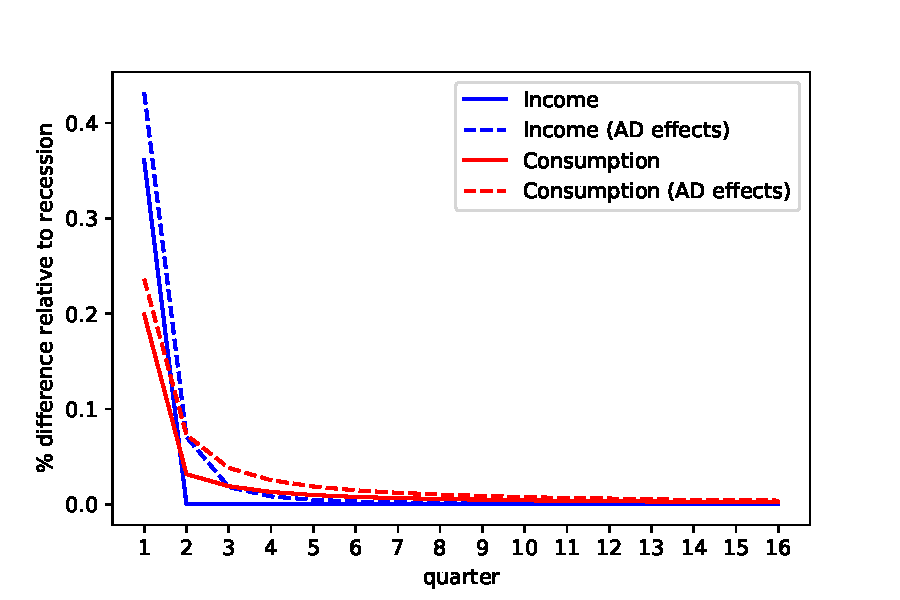
\includegraphics[width=\linewidth]{\PathToRoot/images/recession_Check_relrecession}
      \caption{Check IRF}
      \whenintegrated{\label{fig:recessioncheckrelrecession}} 
    \end{subfigure}
    \hfill%
    \begin{subfigure}[b]{.32\linewidth}
      \centering
      % Original path: \PathToRoot/Code/HA-Models/FromPandemicCode/Figures/recession_UI_relrecession
      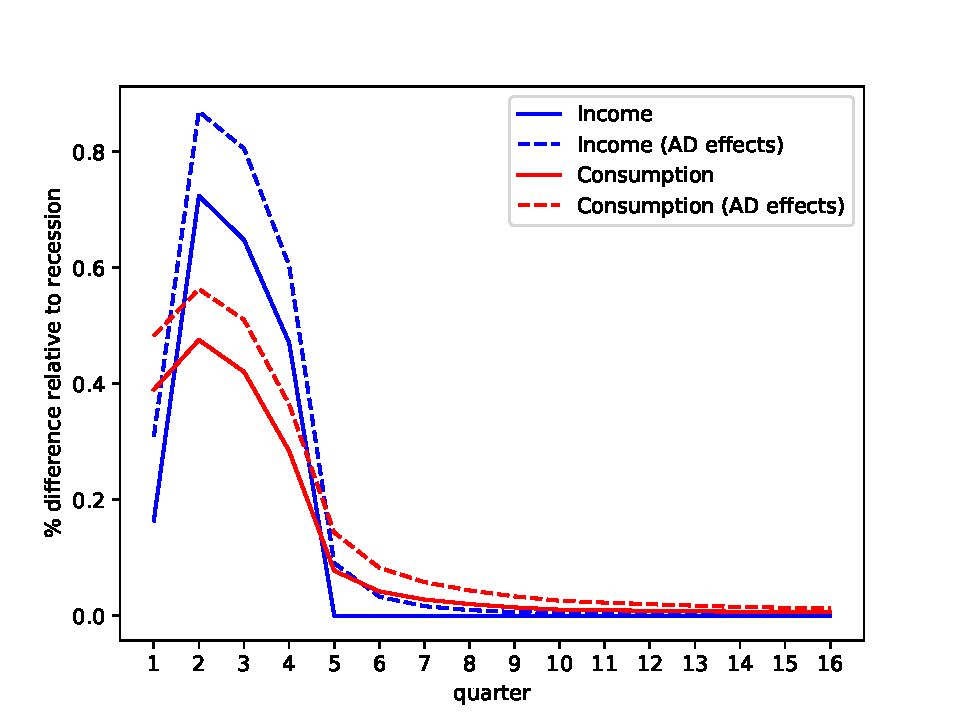
\includegraphics[width=\linewidth]{\PathToRoot/images/recession_UI_relrecession}
      \caption{UI extn IRF}
      \whenintegrated{\label{fig:recessionuirelrecession}} 
    \end{subfigure}
    \hfill%
    \begin{subfigure}[b]{.32\linewidth}
      \centering
      % Original path: \PathToRoot/Code/HA-Models/FromPandemicCode/Figures/recession_taxcut_relrecession
      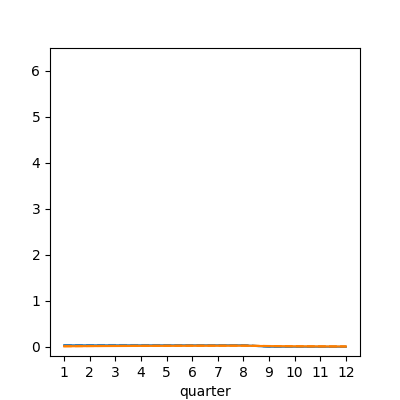
\includegraphics[width=\linewidth]{\PathToRoot/images/recession_taxcut_relrecession}
      \caption{tax cut IRF}
      \whenintegrated{\label{fig:recessiontaxcutrelrecession}} 
    \end{subfigure}
    \\[1.5em]
    \begin{subfigure}[b]{.32\linewidth}
      \centering
      % Original path: \PathToRoot/Code/HA-Models/FromPandemicCode/Figures/Cumulative_multiplier_Check
      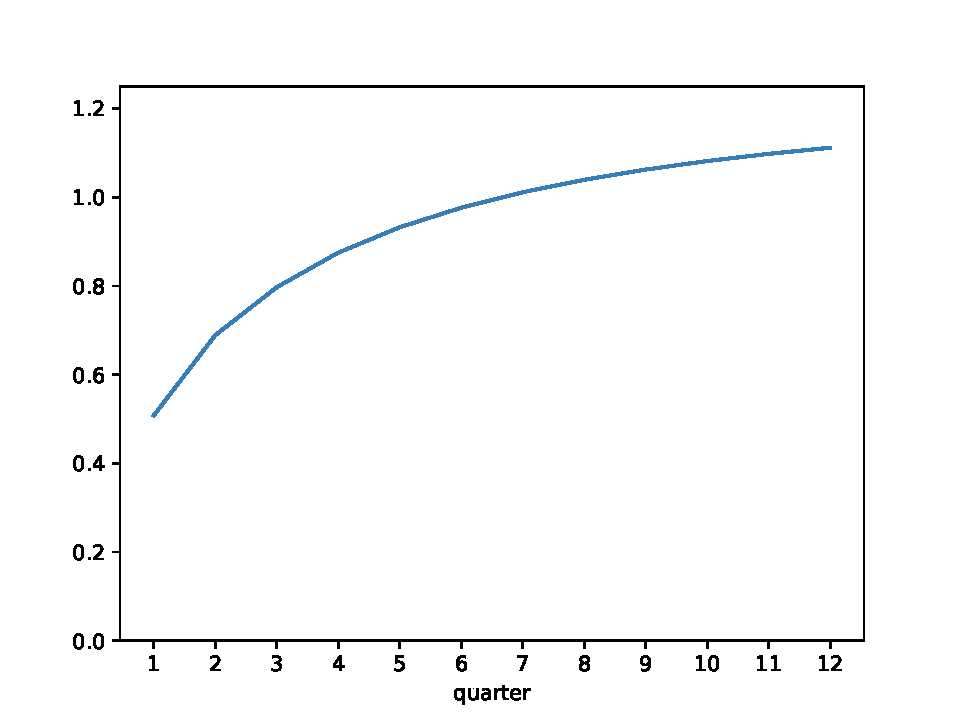
\includegraphics[width=\linewidth]{\PathToRoot/images/Cumulative_multiplier_Check}
      \caption{Check multiplier}
      \whenintegrated{\label{fig:recessioncheckrelrecession_Mult}} 
    \end{subfigure}
    \hfill%
    \begin{subfigure}[b]{.32\linewidth}
      \centering
      % Original path: \PathToRoot/Code/HA-Models/FromPandemicCode/Figures/Cumulative_multiplier_UI
      \includegraphics[width=\linewidth]{\PathToRoot/images/Cumulative_multiplier_UI}
      \caption{UI extn multiplier}
      \whenintegrated{\label{fig:recessionuirelrecession_Mult}} 
    \end{subfigure}
    \hfill%
    \begin{subfigure}[b]{.32\linewidth}
      \centering
      % Original path: \PathToRoot/Code/HA-Models/FromPandemicCode/Figures/Cumulative_multiplier_TaxCut
      \includegraphics[width=\linewidth]{\PathToRoot/images/Cumulative_multiplier_TaxCut}
      \caption{tax cut multiplier}
      \whenintegrated{\label{fig:recessiontaxcutrelrecession_Mult}} 
    \end{subfigure}
  \end{minipage}
\end{figure}
\noindent\parbox{\textwidth}{\footnotesize
  \textbf{Note}: This figure compares policy effectiveness during recessions (Section~\ref{sec:recessions}).
  Recession periods are characterized by higher unemployment rates and increased economic uncertainty.
  The model demonstrates that UI extensions become particularly effective during recessions due to
  better targeting of high-MPC households. Stimulus checks maintain effectiveness but with diminished
  relative performance compared to UI extensions. Payroll tax cuts show the least effectiveness
  across all economic conditions, confirming the robustness of the main policy rankings.
}

% Add clear separation from following content
\vspace{1em}
\FloatBarrier 

% Smart bibliography: Only include bibliography if standalone AND has citations
\smartbib

\end{document}
